%!TEX TS-program = xelatex
\documentclass[12pt, a4paper]{article}\usepackage[]{graphicx}\usepackage[]{color}
%% maxwidth is the original width if it is less than linewidth
%% otherwise use linewidth (to make sure the graphics do not exceed the margin)
\makeatletter
\def\maxwidth{ %
  \ifdim\Gin@nat@width>\linewidth
    \linewidth
  \else
    \Gin@nat@width
  \fi
}
\makeatother

\definecolor{fgcolor}{rgb}{0.345, 0.345, 0.345}
\newcommand{\hlnum}[1]{\textcolor[rgb]{0.686,0.059,0.569}{#1}}%
\newcommand{\hlstr}[1]{\textcolor[rgb]{0.192,0.494,0.8}{#1}}%
\newcommand{\hlcom}[1]{\textcolor[rgb]{0.678,0.584,0.686}{\textit{#1}}}%
\newcommand{\hlopt}[1]{\textcolor[rgb]{0,0,0}{#1}}%
\newcommand{\hlstd}[1]{\textcolor[rgb]{0.345,0.345,0.345}{#1}}%
\newcommand{\hlkwa}[1]{\textcolor[rgb]{0.161,0.373,0.58}{\textbf{#1}}}%
\newcommand{\hlkwb}[1]{\textcolor[rgb]{0.69,0.353,0.396}{#1}}%
\newcommand{\hlkwc}[1]{\textcolor[rgb]{0.333,0.667,0.333}{#1}}%
\newcommand{\hlkwd}[1]{\textcolor[rgb]{0.737,0.353,0.396}{\textbf{#1}}}%
\let\hlipl\hlkwb

\usepackage{framed}
\makeatletter
\newenvironment{kframe}{%
 \def\at@end@of@kframe{}%
 \ifinner\ifhmode%
  \def\at@end@of@kframe{\end{minipage}}%
  \begin{minipage}{\columnwidth}%
 \fi\fi%
 \def\FrameCommand##1{\hskip\@totalleftmargin \hskip-\fboxsep
 \colorbox{shadecolor}{##1}\hskip-\fboxsep
     % There is no \\@totalrightmargin, so:
     \hskip-\linewidth \hskip-\@totalleftmargin \hskip\columnwidth}%
 \MakeFramed {\advance\hsize-\width
   \@totalleftmargin\z@ \linewidth\hsize
   \@setminipage}}%
 {\par\unskip\endMakeFramed%
 \at@end@of@kframe}
\makeatother

\definecolor{shadecolor}{rgb}{.97, .97, .97}
\definecolor{messagecolor}{rgb}{0, 0, 0}
\definecolor{warningcolor}{rgb}{1, 0, 1}
\definecolor{errorcolor}{rgb}{1, 0, 0}
\newenvironment{knitrout}{}{} % an empty environment to be redefined in TeX

\usepackage{alltt}

%%%%%%%%%% Математика %%%%%%%%%%
\usepackage{amsmath,amsfonts,amssymb,amsthm,mathtools}

%%%%%%%%%%%%%%%%%%%%%%%% Шрифты %%%%%%%%%%%%%%%%%%%%%%%%%%%%%%%%%
\usepackage{fontspec}         % пакет для подгрузки шрифтов
\setmainfont{Arial}   % задаёт основной шрифт документа

% Чтобы пропечатывались длинные тире, непрерывные пробелы и тп
\defaultfontfeatures{Mapping=tex-text}

% why do we need \newfontfamily:
% http://tex.stackexchange.com/questions/91507/
\newfontfamily{\cyrillicfonttt}{Arial}
\newfontfamily{\cyrillicfont}{Arial}
\newfontfamily{\cyrillicfontsf}{Arial}

\usepackage{unicode-math}     % пакет для установки математического шрифта
\setmathfont{Asana Math}      % шрифт для математики
% \setmathfont[math-style=ISO]{Asana Math}
% Можно делать смену начертания с помощью разных стилей

% Конкретный символ из конкретного шрифта
% \setmathfont[range=\int]{Neo Euler}

\usepackage{polyglossia}      % Пакет, который позволяет подгружать русские буквы
\setdefaultlanguage{russian}  % Основной язык документа
\setotherlanguage{english}    % Второстепенный язык документа
% Разные мелочи для русского языка из пакета babel
\setkeys{russian}{babelshorthands=true}


\usepackage[paper=a4paper,top=13.5mm, bottom=13.5mm, left=16.5mm, right=13.5mm, includefoot]{geometry}
\usepackage[unicode,colorlinks=true,urlcolor=blue,hyperindex,breaklinks]{hyperref}

\usepackage{indentfirst} % установка отступа в первом абзаце главы!!!
\usepackage{booktabs} 
\usepackage{float}
\usepackage{ifthen}
\usepackage{xstring}

\newcommand{\compr}[1]{
\IfStrEq{#1}{TRUE}{
наш прогноз хороший, так как гипотеза о том, что число пробитий не превышает 5\%, не отвергается. Прогноз заверен Купиком!}{прогноз недостаточно хорош, так как гипотеза о том, что число пробитий не превышает 5\%, отвергается.}}
\IfFileExists{upquote.sty}{\usepackage{upquote}}{}
\begin{document}





\thispagestyle{empty} % Чтобы избежать нумерации титульника

\begingroup

\begin{center}
\small \bfseries ОАО "Очень серьезный банк"
\end{center}

\vfill


\noindent\small Отдел оценки финансовых рисков
\hfill

\begin{center}\bfseries
\large
Ежедневный отчет по значению VaR \\
по всем серьезным и не очень  ценным бумагам
\end{center}

\vfill

\noindent\normalsize
Старшний риск менеджер

\noindent
Винни-Пух
\hfill /\rule{6em}{0.5pt}/\rule{6em}{0.5pt}/

\hfill\makebox[13em]{\hfill\footnotesize (подпись) \hfill\hfill (дата) \hfill}

\noindent
руководитель отдела

\noindent
Ослик Иа
\hfill /\rule{6em}{0.5pt}/\rule{6em}{0.5pt}/

\hfill\makebox[13em]{\hfill\footnotesize (подпись) \hfill\hfill (дата) \hfill}



\vfill

\begin{center}
\normalsize \bfseries Город умных зверей \\ 2017 г.
\end{center}
\endgroup 

\newpage

В данном отчете расчитывается показатель VaR - Value at Risk. Расчеты произведены на основе нормального распределения и проверны с помощью теста Купика.



Ниже представлены динамики цены (см. график \ref{price}) и доходности (cм. график \ref{income}) репрезентативного представителя портфеля "Tesla".

\begin{figure}[h!]
\begin{knitrout}
\definecolor{shadecolor}{rgb}{0.969, 0.969, 0.969}\color{fgcolor}

{\centering 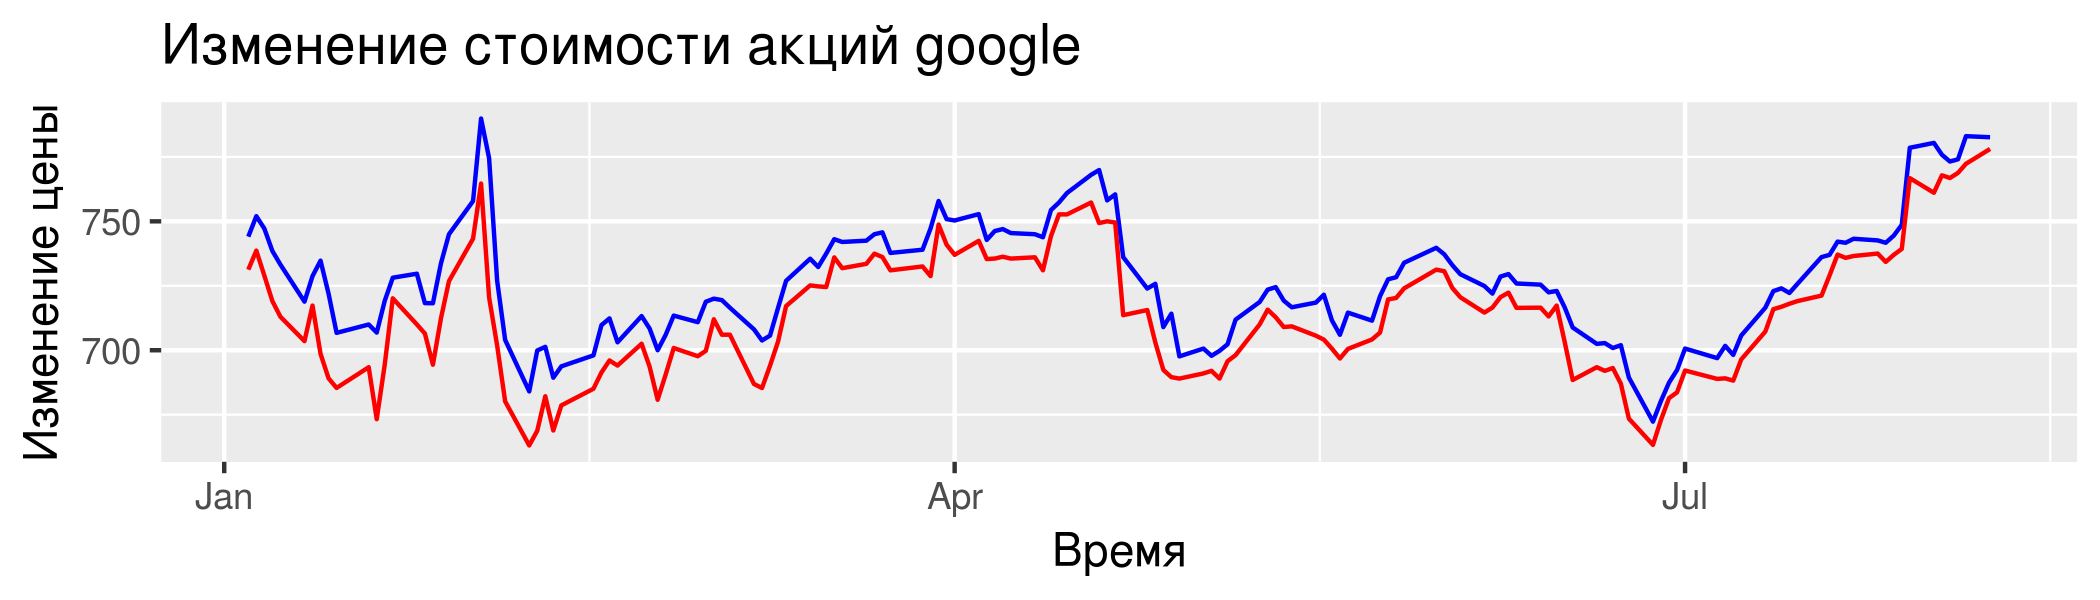
\includegraphics[width=\maxwidth]{figure/unnamed-chunk-3-1} 

}



\end{knitrout}
\caption{Изменение стоимости акций Tesla \label{price}}
\end{figure}




\begin{figure}[h!]
\begin{knitrout}
\definecolor{shadecolor}{rgb}{0.969, 0.969, 0.969}\color{fgcolor}

{\centering 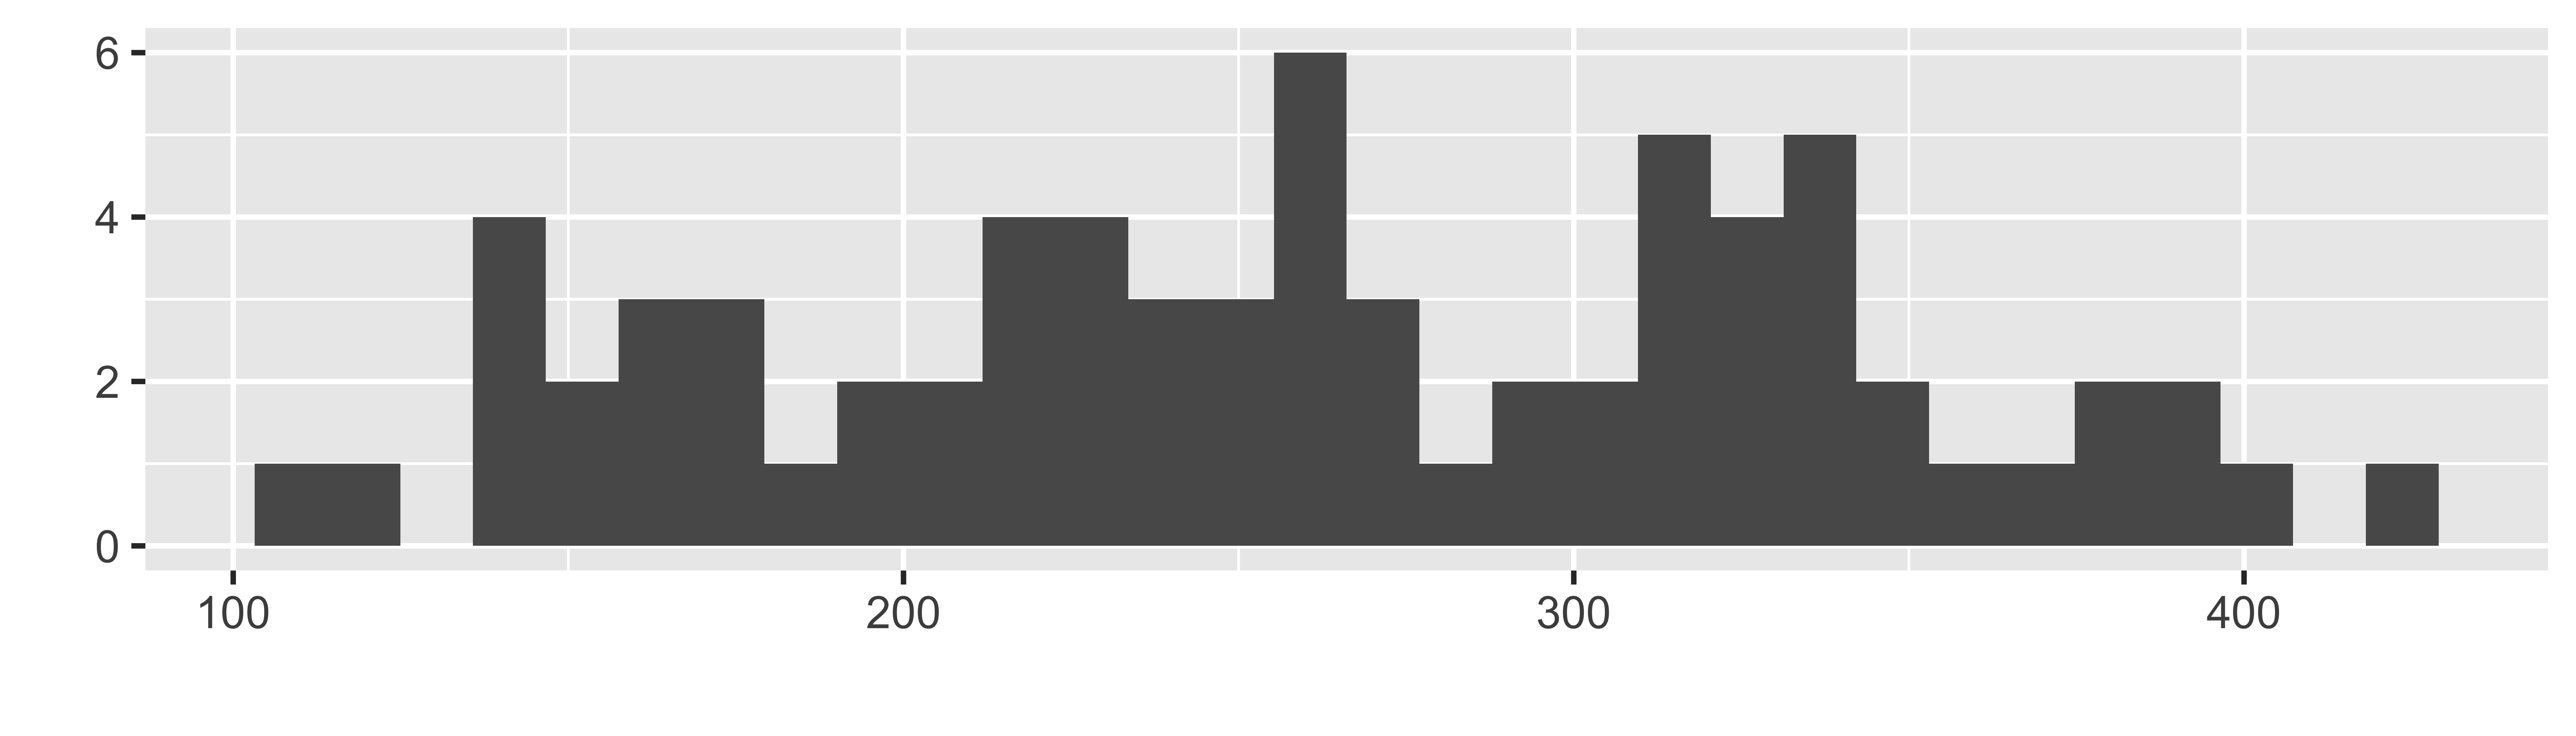
\includegraphics[width=\maxwidth]{figure/unnamed-chunk-5-1} 

}



\end{knitrout}
\caption{Изменение доходностей акций Tesla\label{income}}
\end{figure}




\newpage

Рассчитанное прогнозное значение VaR составляет -0.0438916. Ниже на графике \ref{VaR} можно ознакомится с кривой VaR.

\begin{figure}[h!]
\begin{knitrout}
\definecolor{shadecolor}{rgb}{0.969, 0.969, 0.969}\color{fgcolor}

{\centering 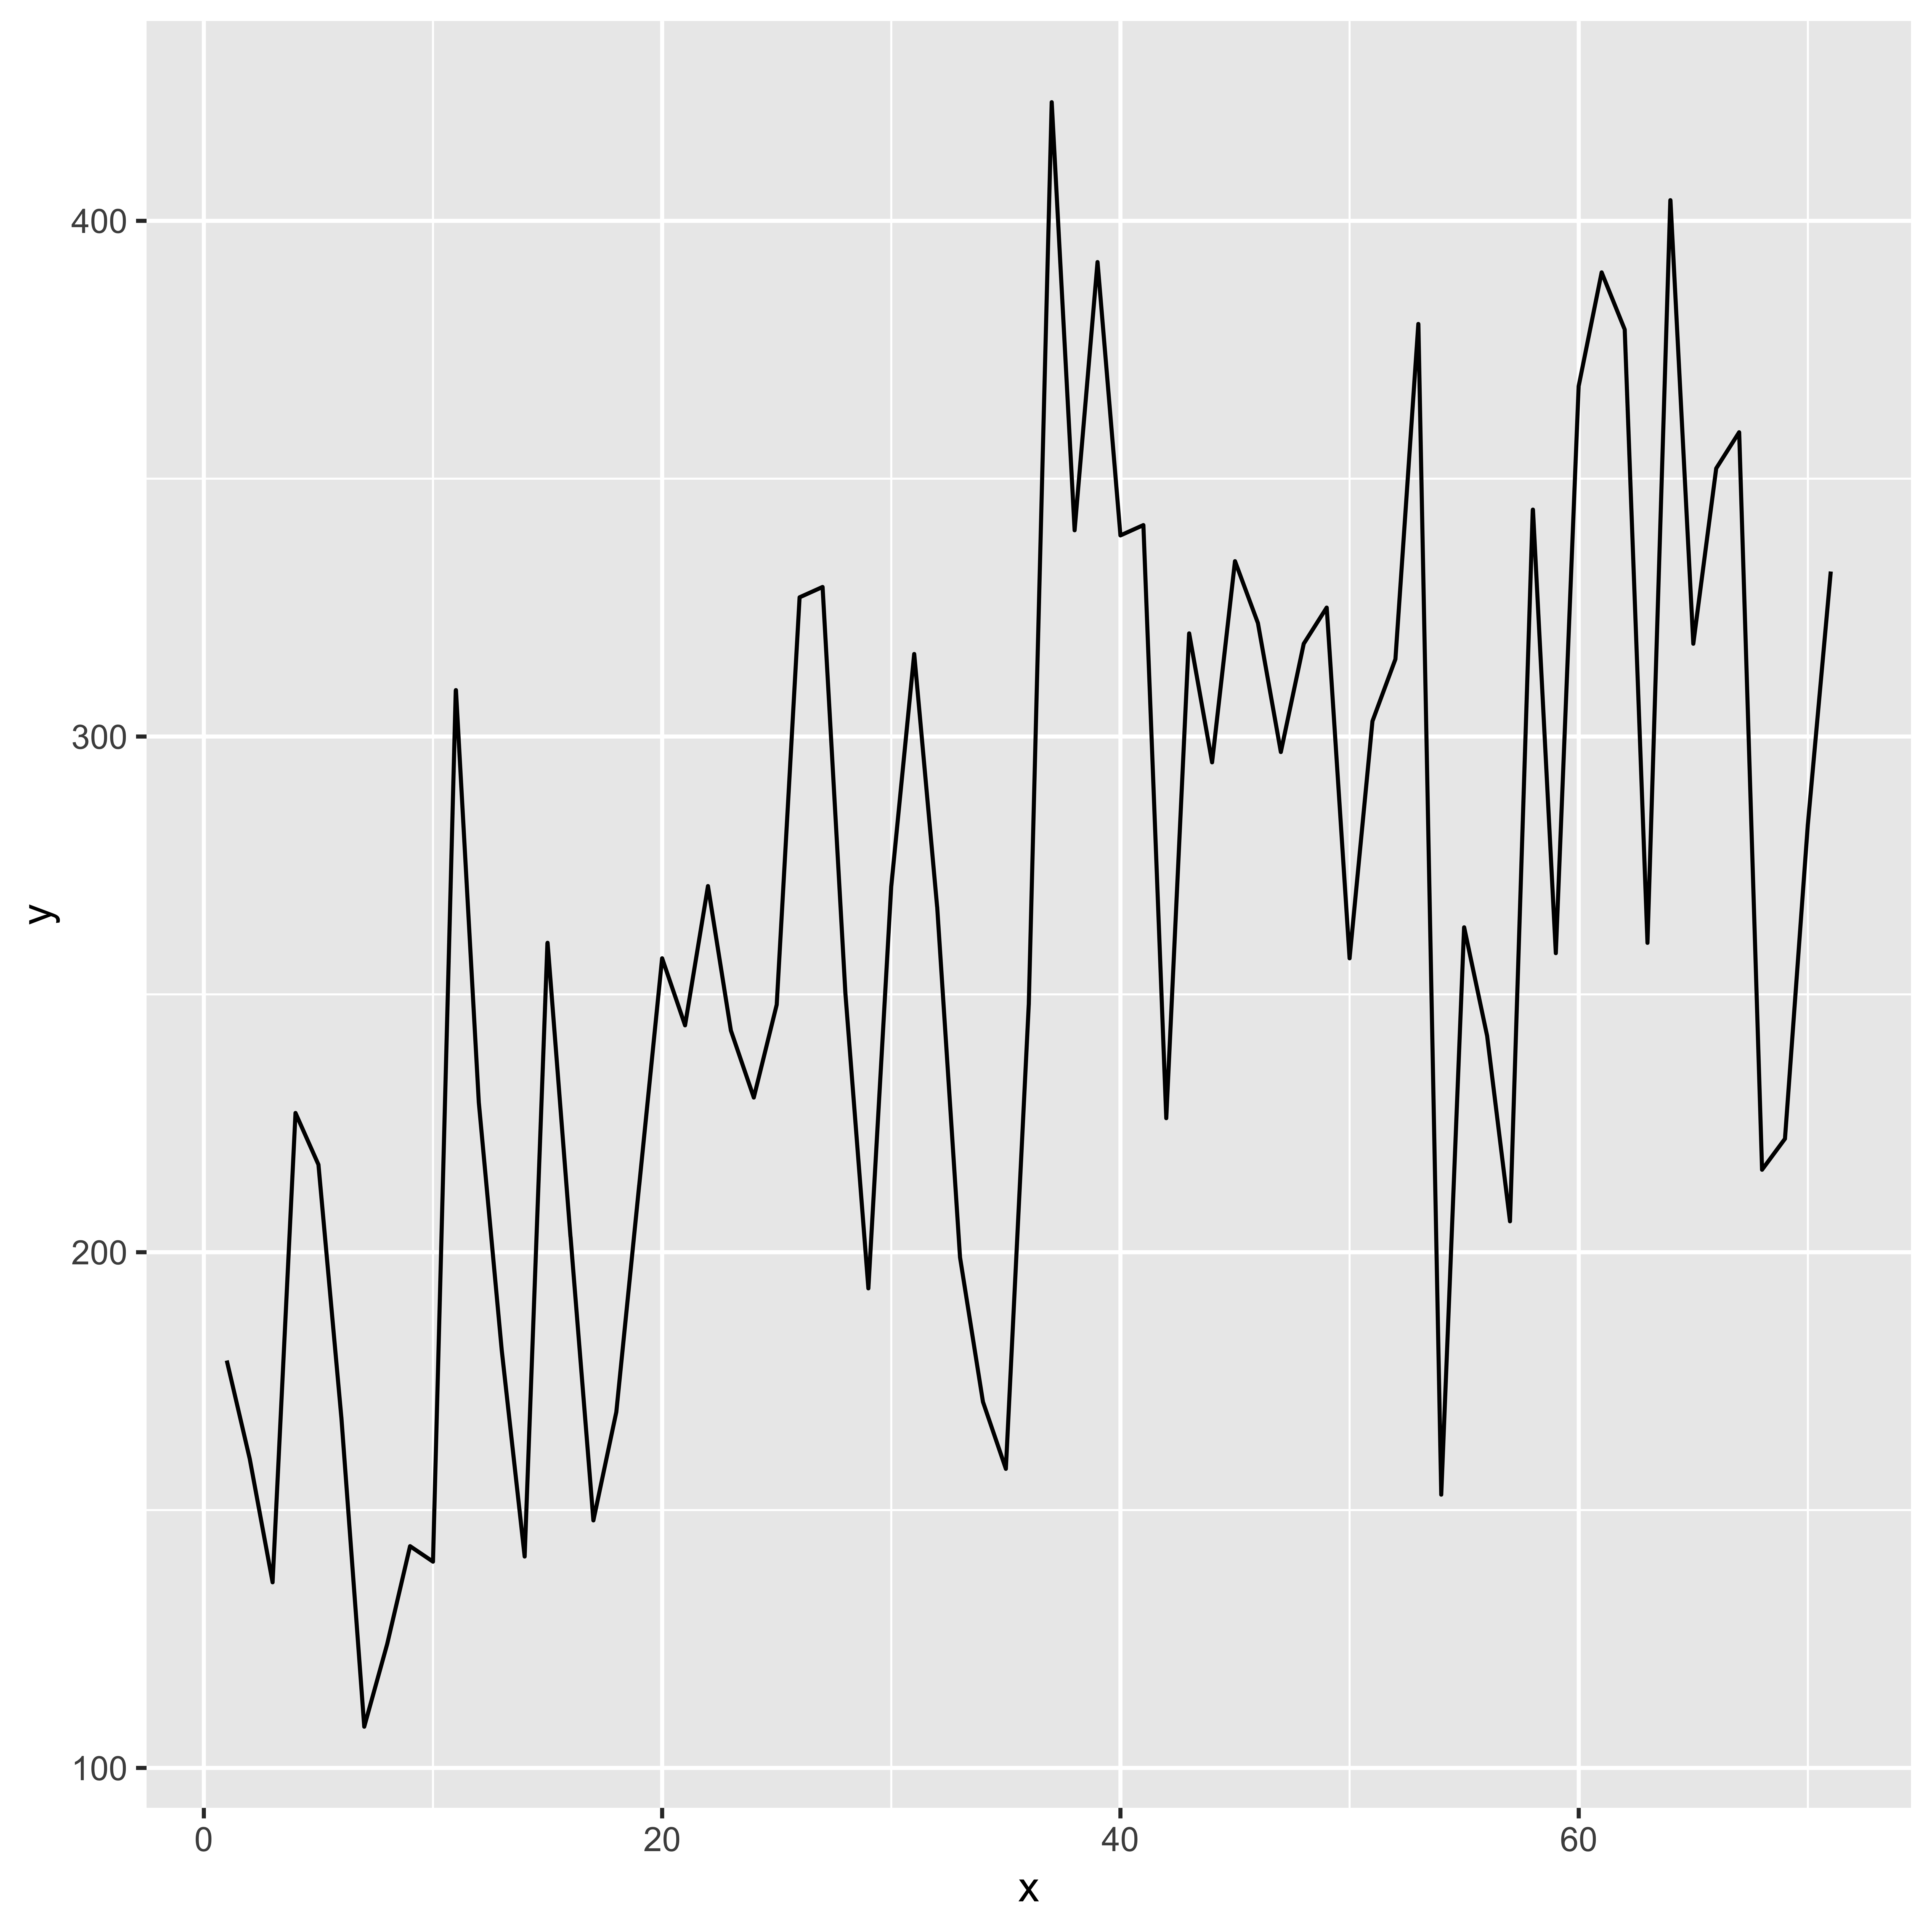
\includegraphics[width=\maxwidth]{figure/unnamed-chunk-7-1} 

}



\end{knitrout}
\caption{Кривая VaR\label{VaR}}
\end{figure}





Как было отмечено выше, проверка адекватности прогноза провидится тестом Купика. Текущее p-value равно 0.2510897, то есть \compr{TRUE}

Результаты проверки гипотезы единичного корня представлены в таблице \ref{tab:unRoot}.




\begin{table}[h!]
\centering
\caption{Augmented Dickey-Fuller Test; stationary \label{tab:unRoot}}
\begin{tabular}{|c|c|c|}
\hline
\textbf{Dickey-Fuller} & \textbf{Lag order} & \textbf{p-value} \\
-7.723248 & 7& 0.01 \\
\hline
\end{tabular}
\end{table}







\end{document}
